\chapter{Implicazioni dell'OSINT nel Dark Web}\label{chapter:Implicazioni}

Mentre il dark web presenta sfide e rischi unici, rimane una fonte essenziale di intelligence per le indagini OSINT, consentendo agli analisti di scoprire minacce nascoste, tracciare attività criminali e migliorare la consapevolezza in un panorama digitale sempre più complesso.

Vediamo ora come questi due strumenti possono interagire, allo scopo di raccogliere e elaborare il maggior numero di dati.

Il dark web svolge un ruolo significativo per quanto riguarda le investigazioni di Open Source Intelligence (OSINT), sempre considerando la sua complessità e i rischi intrinseci. Vediamo alcuni punti chiave che evidenziano l'importanza del dark web per l'OSINT:

\textbf{Accesso a informazioni nascoste:} Il dark web contiene molti dati non indicizzati sui motori di ricerca tradizionali. Ciò include forum, marketpalce e altre piattaforme dove diversi utenti prendono parte in attività illecite, come la vendita di dati rubati, droghe e armi. Gli analisti OSINT possono accedere a queste informazioni per raccogliere dati non presente sui canali o sui browser convenzionali.


\textbf{Monitoraggio di Attività Criminali:} Le forze dell'ordine e gli analisti di cybersecurity monitorano frequentemente il dark web per tracciare attività criminali, tra cui attacchi informatici, frodi e terrorismo. Infiltrandosi in forum e mercati del dark web, gli investigatori possono raccogliere informazioni su potenziali minacce e reti criminali, aiutando nella prevenzione e per sventare attività illegali.

\textbf{Identificazione delle minacce:} Gli analisti OSINT utilizzano il dark web per identificare e profilare gli utenti che cercano di portare a termine diversi crimini, inclusi hacker, criminali informatici e gruppi estremisti. Monitorando i canali di comunicazione e osservando le interazioni tra di essi, gli analisti possono scoprire informazioni preziose su questi individui o gruppi, come le loro tattiche e tecniche.

\textbf{Monitoraggio dei Data Breaches:} Il dark web è un punto caldo per la vendita e lo scambio di dati rubati, tra cui informazioni personali, registri finanziari e credenziali. Le indagini OSINT possono prevedere il monitoraggio dei mercati presenti sul dark web per identificare violazioni dei dati e valutare l'impatto su individui e organizzazioni. Queste informazioni possono essere cruciali per l'incident response e limitare i rischi.


\textbf{Ricerca e Analisi:} Oltre alle attività criminali, il dark web offre un terreno fertile per la ricerca e l'analisi su vari temi, tra cui minacce alla sicurezza informatica, economie sotterranee e tendenze emergenti. Gli analisti OSINT utilizzano strumenti e tecniche per navigare in modo sicuro nel dark web ed estrarre informazioni preziose per definire strategie e per valutare le minacce.

\textbf{Sfide e Rischi:} Nonostante la sua utilità, condurre indagini OSINT sul dark web presenta sfide e rischi importanti. Navigare attraverso i servizi nascosti richiede infatti strumenti e competenze di alto livello, per mantenere l'anonimato e la sicurezza operativa è fondamentale evitare di essere rilevati dagli avversari. Inoltre, l'interazione con le comunità presenti sul dark web comporta considerazioni etiche e legali che devono essere gestite con attenzione.


\section{Monitoraggio delle Minacce}\label{sec:cap_sec_impl1}

Monitorare le attività e i propri dati permette di tracciare minacce e informazioni personali sul Dark Web.
Sorvegliando i forum, i mercati e i servizi di messaggistica del dark web, gli investigatori possono approfondire le tendenze relative al traffico di droga, ai crimini finanziari, al furto di identità, alla vendita di armi, alla tratta di esseri umani e altro ancora. 
Per verificare la validità degli indizi e dei dati rilevati è possibile utilizzare piattaforme del dark web per verificare o smentire informazioni provenienti dal web di superficie, migliorando la credibilità degli indizi investigativi. Infine per contrastare le Minacce Interne è necessario identificare casi di data breach e scambiati sul dark web, questo aiuta a combattere le minacce interne e a rafforzare le misure di sicurezza informatica.

Le minacce possono essere furti di credenziali bancarie, numeri, email e altri dati personali sensibili(allo scopo di appropriarsi dell'identità di un altro utente). 

Le attività di monitoring sono essenziali per due motivi in particolare:
\begin{enumerate}
    \item Perché i data breach sono spesso silenziosi, ovvero le imprese non si rendono immediatamente conto di aver subito un attacco;  
    \item Perché scoprire per tempo una fuga di dati permette di mitigare il danno ed evitare che si ripropongano situazioni analoghe in futuro.
\end{enumerate}

Se a tutto ciò si aggiunge un costo medio di data breach superiore ai 4 milioni di dollari – come suggerisce l’ultimo report IBM sul tema – ci si rende conto non solo dell’importanza del dark web monitoring, ma anche della sua urgenza. 
Il tutto si traduce nella necessità di monitoraggio costante dei siti e delle piattaforme del dark web finalizzata a collezionare informazioni che dimostrino all’azienda di aver subito un data breach.

In questa prospettiva, i tool di monitoraggio del dark web, disponibili come soluzioni stand-alone, software open source o parte integrante di piattaforme di sicurezza, esplorano il dark web per creare database di informazioni che permettano alle aziende di individuare se sono state vittime di violazioni dati o meno.

Non esiste un’indicizzazione unica, affidabile e sicura (come Google, per intenderci) dei servizi del dark web, e oltretutto il crawling dei portali pubblici non è sufficiente; occorre quindi registrarsi, ed interagire fino a aver conquistato la fiducia dei gestori dei siti stessi, che talvolta sono board dedicate allo scambio di informazioni.\cite{implic1}

Il mondo dei tool di dark web monitoring è estremamente ampio e dinamico. Realizzare da zero una soluzione dedicata è una strada difficilmente percorribile, perché oltre alle competenze specialistiche, è necessario l’accesso a fonti riservate e una conoscenza approfondita di piattaforme, siti, marketplace e dei canali.
Alcuni tool per il monitoring quindi possono essere OnionScan, BlackWidow\footnote{OnionScan, per ricercatori e investigatori che monitorano e tracciano i siti del Dark Web e BlackWidow un tool che parte da un sito target e ne effettua scansione e mappatura completa}, il dark web monitoring di NordVPN e Brandefense per la ricerca di informazioni su data breach. Infine piattaforme di cyber threat intelligence come IntSights. 
\newpage

\begin{figure}[h]
	\centering
	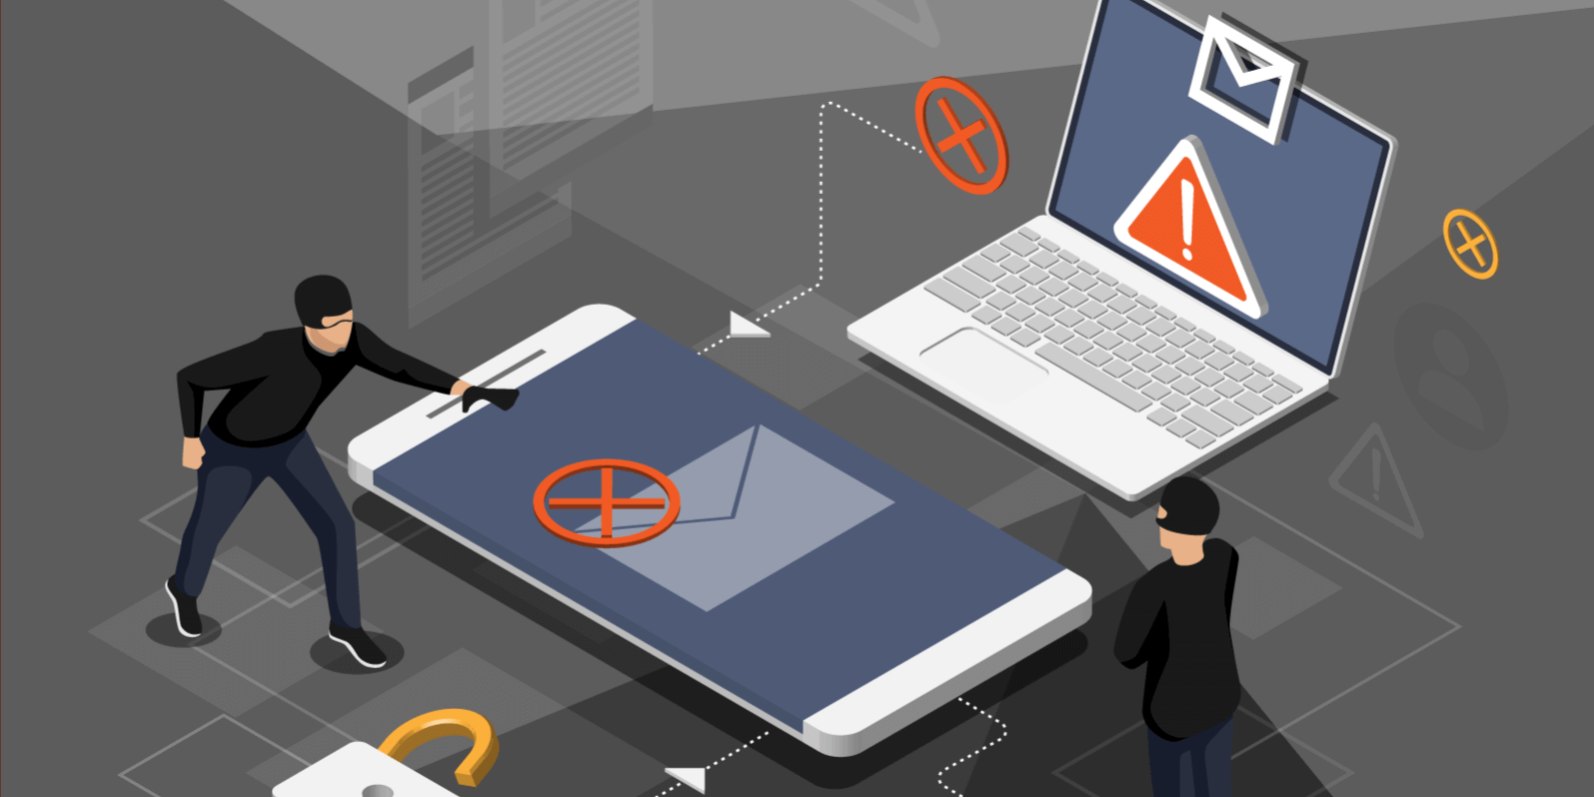
\includegraphics[width=0.8\textwidth]{Immagini/implicazione1.png}
	\caption{Dark Web Monitoring}
	\label{fig:oneimplic}
\end{figure}

Da sottolineare inoltre che il monitoraggio regolare dei propri dati personali, conti di credito e delle transazioni con carte di debito può aiutare a rilevare rapidamente qualsiasi attività non autorizzata e ad agire per prevenire le frodi.

Un altro strumento molto utile è il Daily Dark Web, sito web, specializzato nell'analisi e nel reportage approfondito delle attività del dark web. La loro copertura include approfondimenti dettagliati dei forum di hacker, dei canali Telegram (su cui avvengono attività illecite) e aggiornamenti da gruppi di ransomware. Il loro approccio va oltre il semplice reportage; Negli ultimi anni, i loro investigatori sono stati in grado di ottenere interviste con noti hacker come USDoD e RansomedVC, offrendo uno sguardo nelle menti e nelle motivazioni che guidano queste figure.


\section{Rilevazione dati}\label{sec:cap_sec_impl2}

La rilevazione dei dati, tramite OSINT sul dark web, presenta principalmente 2 difficoltà:

\textbf{Accessibilità Limitata:} La mancanza di indicizzazione dei motori di ricerca e i frequenti cambiamenti di indirizzo del dark web pongono ostacoli alla ricerca e al tracciamento efficiente delle prove, che possono rapidamente scomparire.

\textbf{Affidabilità delle Informazioni:} Le informazioni provenienti dal dark web potrebbero non essere sempre affidabili o accurate, rendendo necessari processi di validazione e verifica accurati. Per mitigare questi rischi, l'investigatore deve utilizzare software specializzati come Tor, utilizzare VPN e aggiornare costantemente i loro strumenti. Inoltre, devono prestare la massima attenzione per evitare di lasciare tracce digitali che potrebbero compromettere la loro identità e l'integrità delle loro indagini.


Per analizzare e interpretare correttamente i dati ottenuti è essenziale avere un approccio sistematico.

\begin{enumerate}
    \item Si deve raccogliere e organizzare il dato in base al tipo, assicurandosi che questo avvenga legalmente e eticamente,
    \item  Verificare e confermare l'informazione, effettuando cross-referencing dei dati con quelli del web di superficie quando possibile,
    \item Identificare Connessioni e Reti, analizzando profili utenti, conversazioni e transazioni, mappando le reti e individuando i protagonisti,
    \item Analizzare i modelli di attacco, identificando tattiche e tecniche, analizzando modelli e metodologie di attacco, allo scopo di migliorare le strategie difensive,
    \item Ricavare Intelligence Attuabile, sintetizzando i risultati, evidenziando informazioni chiave, tendenze e assicurare la tempestiva diffusione dell'intelligence,
    \item E mantenere la sicurezza operativa, implementando misure rigorose per la gestione e la protezione dei dati, utilizzando software specifici e applicando procedure di audi adeguate.
\end{enumerate}


Ritroviamo diverse tipologie di dati ricavabili dal Dark Web, di seguito quelli di rilievo:
\\
\textbf{\\Profili utenti
\\Conversazioni
\\Transazioni (Crypto)
\\Attività illecite (vendita di articoli illegali)
\\Denunce e altri dati
\\Annunci da Marketplace
\\Connessioni (tra utenti, gruppi e organizzazioni)
\\Dati sensibili (Password e informazioni personali)}

\section{Vendita di Informazioni}\label{sec:cap_sec_impl3}

Agli investimenti in cyber security spesso viene data poca importanza all'interno dell'aziende, il più delle volte per questioni legate a un presunto risparmio. Invece abbiamo visto, che proteggere il patrimonio informativo ed evitare fughe di notizie causate da attacchi di social engineering dovrebbero essere tra i principali obbiettivi. 
Anche perché, i dati sottratti a aziende passano inevitabilmente attraverso il mercato nero del Dark Web.

Chi si appropria dei dati, con ogni probabilità non ne sarà l'utlizzatore diretto, bensì verranno rivenduti nei canali underground della rete.

Funzionamento dei marketplace:

Troviamo all'interno di questi siti uno degli elementi più costosi e ricercati, il malware premium, che può arrivare a costare cinquemila dollari (per mille installazioni). Altri listing sui siti possono comprendere, dati di accesso ad account PayPal (spesso non funzionanti grazie all’autenticazione a due fattori), accessi Netflix o dettagli di carte di credito rubate.

In questi marketplace riscontriamo spesso tentativi di frode, che possiamo indicare in tre macro categorie:

La prima è relativa alla classica truffa in cui un'utente paga per l’acquisto di un determinato bene che mai arriverà nelle proprie mani;
La seconda riguarda il pagamento per l’acquisto di materiale, il quale non risulterà conforme alle fotografie, ad esempio nel caso di documenti falsi;
La terza categoria, infine, riguarda la truffa in cui, viene pagata una cifra molto elevata, per articoli e dati che l'utente sarebbe stato in grado di reperire a prezzi più convenienti, sul web di superficie.

\'E consigliabile quindi non favorire e non prendere parte a queste tipologie di transazioni.

Tuttavia, è sorprendente notare come le guide alle frodi e all’hacking siano alcuni degli articoli più venduti.

Le guide pratiche sulle truffe che includono tutorial su come eseguire attività dannose risultano le più vendute per il cinquanta per cento, seguite dalle vendite di dati personali e data Breaches\footnote{comprendono nomi, numeri di telefono, indirizzi, indirizzi e-mail e codici fiscali}.

Inoltre, troviamo anche diversi account e credenziali non finanziari, che includono account per servizi come Amazon, PayPal, Stripe, Kraken e altri media bancari e di cripto valuta.

Infine, ritroviamo strumenti e modelli di frode, i quali includono applicazioni che possono essere utilizzate come trojan\footnote{Indica un tipo di malware, in cui come il cavallo dell'antica storia greca, si nasconde all'interno di un altro programma apparentemente utile e innocuo} e siti web preconfezionati per attacchi di tipo phishing.\cite{implic2}


\section{Analisi di Comunità Online}\label{sec:cap_sec_impl4}

I Marketplace più comuni, utilizzati per le investigazioni OSINT comprendono AlphaBay, Empire Market, e Silk Road (o i suoi successori, in quanto successivamente a diverse operazioni delle forze dell'ordine e dell'FBI, molti di questi siti sono stati sequestrati e chiusi). Queste comunità facilitano lo scambio di beni e servizi illeciti e forniscono informazioni preziose agli investigatori.

Oltre ai marketpalace il Dark Web ospita una miriade di forum che operano al di fuori dei siti web convenzionali, fungendo da epicentri per attività di cybercriminalità. Questi forum non sono solo luoghi d'incontro per hacker e attori illeciti; sono ecosistemi dove dati rubati, strumenti di hacking e servizi vengono scambiati.

Qui ritroviamo forum come BreachForums e XSS, che offrono uno sguardo nel sofisticato mondo delle minacce informatiche e dei data breaches. Queste piattaforme, avvolte nell'anonimato, sono luoghi in cui i confini della legalità si confondono, mettendo alla prova gli sforzi di cybersicurezza a livello globale. Analizziamo le loro operazioni, i loro membri e l'impatto complessivo che hanno sia nel mondo cibernetico che in quello fisico.

\begin{figure}[h]
	\centering
	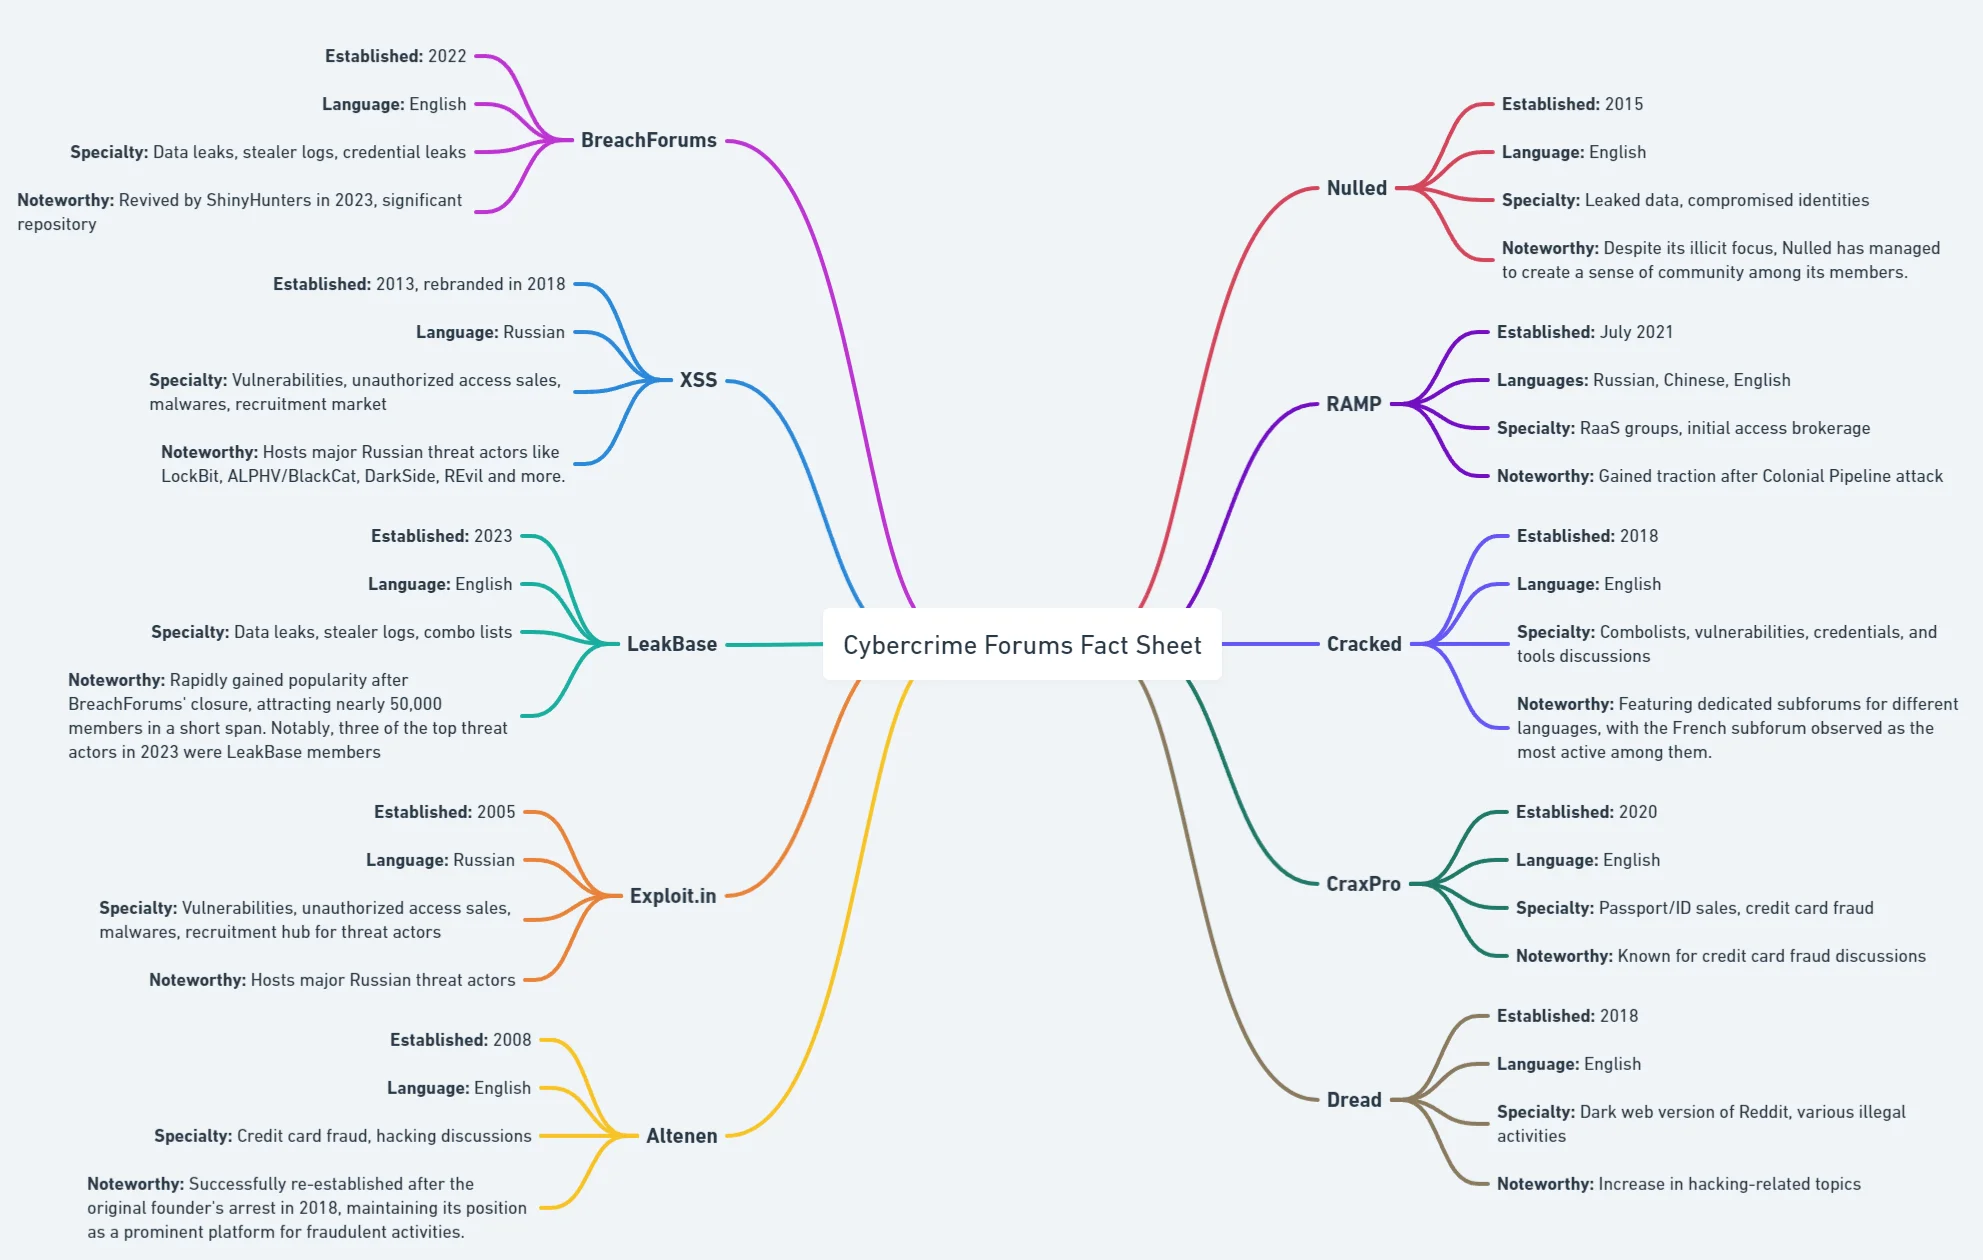
\includegraphics[width=1\textwidth]{Immagini/implicazione2.jpg}
	\caption{Principali forum dal Dark Web}
	\label{fig:twoimplic}
\end{figure}

\newpage
\paragraph{Forum principali e come forum e come operano:}

\begin{enumerate}
    \item \textbf{BreachForums:}
    \\BreachForums è emerso rapidamente come uno dei temi mainstream sui forum del dark web, specialmente dopo la chiusura di RaidForums e la sua sostituzione con quest'ultima. La storia iniziò quando un noto hacker, Pompompurin, lanciò Breached dopo la scomparsa di RaidForums.

    Una sequenza di avvenimenti ha portato all'arresto di Pompompurin da parte delle forze dell'ordine statunitensi, il 15 marzo 2023, la chiusura di Breached (noto anche come BreachForums) non ha segnato la fine del forum. Al contrario, un nuovo team ha rilanciato il forum sotto il nome di BreachForums, diventando rapidamente il fulcro del dark web e riuscendo dove altri forum avevano fallito.

    Il 12 giugno 2023, BreachForums ritorna sotto il nome di ShinyHunters, e si conferma come uno dei gruppi più attivi. Nonostante lo scetticismo iniziale sulla sua legittimità, con diversi utenti che temevano fosse una trappola dell'FBI, un messaggio firmato con PGP da un ex amministratore, Baphomet, ne conferma il ritorno. ShinyHunters, noto per significativi data breaches alle spese di aziende come Tokopedia e GitHub, ha continuato ad attirare l'attenzione per la vendita di dati rubati, evidenziando le costanti sfide in materia di cybersecurity e protezione dei dati.

    BreachForums si distingue per i suoi database admin-approved, vantando oltre 15 miliardi di record provenienti da 936 dataset e una serie di sezioni particolarmente attive del forum, tra cui Leaks, Stealer Logs e il suo ranking system (VIP, MVP, GOD), insieme a un sistema di punti di credito, all'interno del forum e bastato sulle transazioni.

    L'importanza del forum, tuttavia, deriva dalla da alcuni dei membri quali, i fondatori e hacker di rilievo.

    \item \textbf{XSS:}
    \\XSS, con una storia che risale al 2013, emerge non solo come uno dei forum più antichi ma anche come un importante hub per hacker competenti nel panorama cyber Russo. Fondato nel 2013, il forum ha subito un rebranding nel 2018, adottando il nome XSS in riferimento alla vulnerabilità Cross-Site Scripting dopo l'arresto di uno dei suoi amministratori nel 2017. Operando sia come piattaforma TOR sia accessibile dal web di superficie, XSS si presenta come un forum hacker dove le discussioni ruotano principalmente attorno alla vendita di credenziali, malware, vulnerabilità di sicurezza e data breach.

    Data la sua base di utenti Russi e la sua notorietà, XSS ha ospitato celebri hacker russi, tra cui LockBit, ALPHV/BlackCat, REvil e il gruppo DarkSide responsabili dell'attacco al Colonial Pipeline\footnote{Un'importante attaco ransomware che prese di mira la Colonial Pipeline Company, il più grande operatore di gasdotti negli Stati Uniti, nel maggio 2021}. Il forum funge da punto di incontro, facilitando annunci di reclutamento e varie transazioni di malware, virus e altri strumenti. I gruppi di Ransomware-as-a-Service (RaaS) e altri hacker utilizzano XSS per scopi di pubbliche relazioni, partecipando a discussioni e promuovendo le loro attività allo scopo di rafforzare la loro reputazione.
    
%\begin{figure}[ht]
%   \centering
%	\includegraphics[width=0.8\textwidth]{Immagini/implicazione3.png}
%	\caption{Timeline Dell'Attacco Colonel Pipeline}
%	\label{fig:threeimplic}
%\end{figure}

    
    \item \textbf{LeakBase:}
    \\LeakBase emerge come uno dei forum più recenti e importanti di questa lista. Si stima sia stata creata nel gennaio 2023, questo forum in lingua inglese è accessibile sul web di superficie e ha rapidamente guadagnato popolarità, soprattutto dopo la chiusura di BreachForums nel marzo 2023. E ha colmato il vuoto creato nel panorama del cyber crime, guadagnandosi una certa notorietà.

    Con un sistema di classificazione simili a BreachForums e il suo sistema di crediti, LeakBase ha attirato l'attenzione, guadagnando quasi 50.000 membri in breve tempo. Il forum evidenzia discussioni su data leaks, stealer logs, combo list, vulnerabilità, malware e persino software legali, ognuno contenuto in una categoria distinta.

    Inoltre, il forum presenta una sezione privata dedicata a contenuti esclusivi ed è vietato condividere informazioni riguardo la Russia.

    \item \textbf{Exploit.in:}
    \\Fondato nel 2005, Exploit si presenta come uno dei principali forum hacker russi nel panorama del cyber crime, simile a XSS. Opera sia su TOR che sul web di superficie, Exploit serve come punto di ritrovo per data dump iniziali, facilitando la vendita di credenziali, la diffusione di malware, data breaches e le transazioni di database, sia per la loro vendita che per la loro distribuzione gratuita.

    Proprio come XSS, Exploit sfrutta la sua capacità nel connettere i cybercriminali con potenziali collaboratori, allo scopo di organizzare attività di hacking, frode o per l'organizzazione di gruppi Ransomware-as-a-Service (RaaS).

    Con la sua organizzazione strettamente strutturata e le sue politiche di adesione, Exploit proietta quasi un'aura di professionalità.

    \item \textbf{Altenen:}
    \\Altenen si distingue dagli altri forum in lingua inglese accessibili sul web di superficie. Focalizzandosi su una varietà di attività fraudolente, in particolare, frode con carte di credito, il forum approfondisce discussioni sulle diverse tecniche, (cracking, hacking, argomenti IT e molto altro).

    Fondato nel 2008, Altenen ha affrontato una battuta d'arresto quando il suo fondatore è stato arrestato nel maggio 2018, ma grazie alla condivisione su social network come X e YouTube, la piattaforma ha continuato ad avere una fanbase molto attiva.

    \item \textbf{Nulled:}
    \\Fondato nel 2015, Nulled è un noto forum cybercriminale in lingua inglese presente prevalente nel dark web. Ospita una varietà di contenuti illeciti, tra cui informazioni personali, identità, informazioni su carte di credito e strumenti per l'hacking. Nonostante il suo focus illegale, viene fatta passare come una comunità per condividere leak e partecipare a semplici discussioni.

    Nel 2016, Nulled è stato reso famoso a causa di un grave data breach che ha esposto informazioni personali di migliaia di utenti. Nonostante i rischi, continua ad essere accessibile sia dal web pubblico che dal dark web, attirando utenti con diversi livelli di accesso.

    \item \textbf{RAMP:}
    Fondato nel luglio 2021, RAMP (Russian Anonymous Market Place) si distingue tra i forum del dark web di lingua russa, cinese e inglese. Il forum mantiene politiche rigorose per l'adesione, con una delle più cruciali, ciò avere una buona reputazione sui altri forum, come XSS e Exploit. RAMP è aumentato in popolarità capitalizzando sugli effetti dell'attacco al Colonial Pipeline negli Stati Uniti, sfruttando i suoi effetti sul dark web.

    Dopo l'attacco al Colonial Pipeline, molti forum hacker hanno imposto restrizioni sui dati, in particolare ai gruppi ransomware. Servendo come punto vitale per i gruppi di Ransomware-as-a-Service (RaaS), RAMP ha poi riservato un'area  nel suo "programma partner" per questi gruppi e per dar loro la possibilità di condurre attività come il reclutamento di nuovi hacker o la vendita di credenziali.

    \item \textbf{Cracked:}
    \\Cracked opera come un forum attivo sul web di superficie. Come lingua principale utilizza l'inglese e le discussioni riguardano prevalentemente dati, vulnerabilità, credenziali e strumenti illeciti. Il forum presenta anche 12 sotto-forum dedicati ad altre lingue, con il sotto-forum in francese che risulta essere il più attivo.

    \item \textbf{CraxPro:}
    \\Fondato nel 2020 è un forum in lingua inglese, all'interno del quale le discussioni ruotano attorno a temi come la vendita di passaporti/ID, la vendita di cookie e credenziali, database, vendita di proxy SOCKS4 e carte di credito. Sebbene l'attività legata alle frodi con carte di credito possa talvolta superare quella di Altenen, gli utenti che le utilizzano suggeriscono che le informazioni sono spesso imprecise.

    \item \textbf{Dread:}
    \\Fondato nel 2018, come lingua principale è utilizzato l'inglese, Dread è stato fondato da un gruppo di hacker, tra cui HugBunter. Viene soprannominato "Reddit del dark web" per la sua interfaccia simile. Dread è uno dei più grandi forum del dark web, bensì i temi di sicurezza, vulnerabilità e intelligence siano presenti, le discussioni sulla vendita di stupefacenti spesso oscurano il resto degli argomenti.
\end{enumerate}
\cite{implic3}


\section{Analisi delle Tendenze e Prevenzione}\label{sec:cap_sec_impl5}

Per verificare e prevenire che le informazioni aziendali non siano state illegalmente pubblicate o sottratte, è possibile svolgere una serie di attività per mantenere protette le informazioni e assicurarsi che lo rimangano:

\textbf{Cercare informazioni con l'utilizzo di OSINT}, determinando quali informazioni l'organizzazione è disposta a rendere pubbliche e se l'organizzazione ha il controllo su queste informazioni. Da queste sarà possibile creare un elenco di tutte le vulnerabilità che eventuali hacker possono utilizzare a loro vantaggio. Sarà in oltre possibile gestire e configurare al meglio i sistemi in modo tale da non divulgare informazioni che non si vuole vengano rese pubbliche.

Sarà poi di primaria importanza una \textbf{continua formazione sulla cybersecurity}. Per identificare vulnerabilità e correggere falle di sicurezza. Addestrando al meglio i dipendenti e preparandoli ad affrontare al meglio potenziali attacchi, investendo in programmi di formazione continua per i dipendenti per migliorare la consapevolezza sulla sicurezza informatica, come il riconoscimento delle email di phishing, la gestione delle password e la risposta agli incidenti. L'elemento umano è spesso l'anello più debole, quindi l'educazione e la sensibilizzazione sono cruciali e infine creando dei SOP (Procedure Operative Standard).\cite{implic4}

Da notare che OSINT è sia un vantaggio che un rischio per la sicurezza di un'organizzazione. In quanto è possibile usare OSINT per identificare punti deboli e migliorare la sicurezza; ma questo permette anche a potenziali hacker di sfruttare le minacce e utilizzare le stesse informazioni per lanciare attacchi mirati ed efficaci. 
Ecco perché è fondamentale che le organizzazioni siano consapevoli dei potenziali rischi associati a OSINT e prendano misure per proteggere le loro informazioni sensibili.

Sarà necessario effettuare un monitoraggio constante delle tendenze, restando aggiornati sulle ultime minacce e collaborando con team di Threat Intelligence per raccogliere informazioni sulle nuove vulnerabilità, attori e "tattiche, tecniche e procedure" (TTP). Utilizzando fonti di OSINT (Open Source Intelligence), dark web monitoring e rapporti fornite da agenzie di sicurezza.


\'E poi fondamentale implementare sistemi di Difesa a più livelli, utilizzando un approccio di difesa in profondità che includa firewall, sistemi di prevenzione delle intrusioni (IPS), antivirus, antimalware, e sistemi di rilevamento delle minacce basati su intelligenza artificiale (per identificare comportamenti anomali, rilevare e rispondere a minacce zero-day e automatizzare la gestione degli incidenti. L'automazione riduce il tempo di risposta e limita l'esposizione alle minacce).

Ulteriori attività di prevenzione:

\begin{enumerate}
    \item Per prevenire futuri attacchi sarà utile simulare attacchi e penetration testing, in quanto condurre regolari test e simulazioni di attacchi (come il Red Teaming) per identificare punti deboli nella rete aziendale e nelle infrastrutture di sicurezza, permetteranno una valutazione realistica della postura di sicurezza dell'organizzazione. Pianificando e preparando Incident Response, sviluppando e mantenendo aggiornato un piano di risposta agli incidenti (IRP) che stabilisca chiare procedure operative per affrontare potenziali violazioni della sicurezza, permetterà ai team di essere sempre preparati.
    \item Ottenere una copertura di assicurazione contro i rischi cyber per mitigare le perdite finanziarie derivanti da attacchi informatici.
    \item Adottare soluzioni di sicurezza per proteggere gli endpoint (laptop, dispositivi mobili, server) e le infrastrutture cloud. Implementare politiche di sicurezza zero-trust, che prevedono il controllo rigoroso degli accessi e la segmentazione della rete.
    \item Stabilire un team di Cyber Threat Hunting per cercare minacce avanzate che potrebbero non essere rilevate dai sistemi di difesa tradizionali.
    \item Monitorare il dark web per rilevare dati aziendali rubati, informazioni sensibili o qualsiasi menzione dell'azienda che potrebbe indicare un attacco imminente. I servizi di monitoraggio dei social media possono aiutare a identificare campagne di phishing o minacce di insider.
    \item Sviluppare un'architettura di sicurezza scalabile che possa crescere con l'azienda. Questo include la protezione delle API, l'uso di DevSecOps\footnote{Development, Security, and Operations è un approccio integrato allo sviluppo del software che incorpora pratiche di sicurezza informatica direttamente nel ciclo di vita dello sviluppo del software (SDLC)} per integrare la sicurezza nello sviluppo del software e la crittografia dei dati sensibili a riposo e in transito.
\end{enumerate}


\section{Minacce Emerse dal Dark Web}\label{sec:cap_sec_impl6}

Utilizzare il dark web per indagini OSINT comporta diversi rischi significativi che richiedono una gestione attenta:\\

\textbf{Esposizione a Contenuti Illegali e Disturbanti:} Il dark web ospita infatti una vasta quantità di materiale illegale e potenzialmente non censurato, presentando dilemmi legali ed etici per gli investigatori.

\textbf{Tracce Digitali:} Gli investigatori devono essere estremamente cauti per evitare di lasciare tracce digitali, che potrebbero compromettere la loro identità e l'indagine. Sono necessarie competenze e strumenti specializzati per accedere al dark web e navigarlo in modo sicuro e anonimo.

\textbf{Sono presenti Informazioni Inaffidabili e potenzialmente sbagliate:} Le informazioni raccolte dal dark web potrebbero non essere sempre affidabili o accurate, richiedendo quindi una valutazione attenta.

\textbf{Struttura non adeguata e Difficoltà di Ricerca:} Il dark web non è indicizzato dai motori di ricerca e gli indirizzi cambiano frequentemente, rendendo difficile la ricerca e il monitoraggio di prove che possono rapidamente scomparire.

\textbf{Potenziali Implicazioni Legali:} Accedere al dark web può comportare rischi legali, poiché un'investigatore potrebbero essere scambiato per un hacker dalle forze dell'ordine.

\textbf{Minacce di Malware e Hacking:} Esistono rischi di sicurezza intrinseci nell'accesso al dark web, come malware e tentativi di hacking che potrebbero interrompere un'indagine e mettere a repentaglio la sicurezza di un'utente.\\

\medskip
\medskip
Per verificare la veridicità dei dati, e limitare il rischio derivante dalle attività sul Dark Web è possibile svolgere le seguenti operazioni:\\

Cross-Reference con risorse dal web pubblico:
\\Confrontando i dati del dark web con le informazioni disponibili sul web pubblico per identificare inconsistenze.
Verificare nomi utente, informazioni di contatto e schemi di attività su più piattaforme.\\

Valutare l'affidabilità delle informazioni sul Dark Web:
\\Valutare la reputazione e la credibilità dei forum del dark web, dei marketplace e dei servizi di messaggistica utilizzati come fonti di dati.\\

Analizzare pattern e anomalie:
\\Cercare schemi nei dati coerenti con attività criminali note, identificare anomalie e incoerenze nei dati e svolgere ulteriori indagini.\\

Utilizzare le informazioni e le risorse di media di divulgazione:
\\Confrontare i dati del dark web con le informazioni provenienti da dai media, migliorando l'affidabilità dei dati.\\

Verificare i dati con gli esperti:
\\Collaborare con le forze dell'ordine, professionisti della cybersecurity e analisti dell'intelligence esperti in indagini sul dark web. Sfruttando la loro esperienza per verificare dati del dark web.\\

In fine verifica che tutti i dati raccolti dal dark web siano stati ottenuti legalmente ed eticamente.